\chapter{仿真实验与一致性测试}
\label{cha:evaluate}


\section{本章引言}
本章主要对RSCP-iBGP系统的功能进行了测试评价、对新系统下的新协议进行了一致性测试。功能验证方面,通过设计合理的网络拓扑,验证RSCP-iBGP系统,实现了路由存储和路由计算的集中优化、在路由计算的过程中基于全部路由且不存在因为MED不可比引起路由震荡等功能。本文提出的RSCP-iBGP新系统对iBGP协议进行了改动,对RSCP-iBGP新系统下的新协议通过TTCN-3测试例进行一致性测试,很好地验证了RSCP-iBGP系统功能实现与设计的一致性。

\section{RSCP-iBGP系统功能验证实验}

\subsection{路由存储集中优化}


\begin{figure}
  \centering
  % Requires \usepackage{graphicx}
  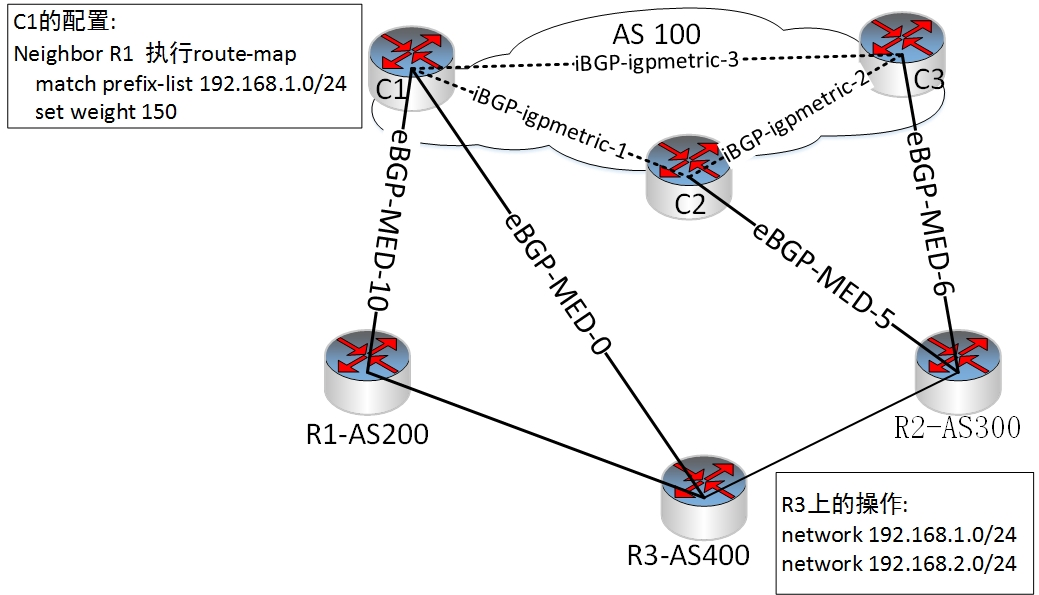
\includegraphics[width=0.75\textwidth]{rscp-example-fm}
  \caption{自治系统内iBGP全连接的网络拓扑图}
  \label{fig:rscp-example-fm}
\end{figure}

在本文提出的RSCP-iBGP系统中,自治系统内的Loc-RIB路由信息均存储在集中平台的Route-Server路由器上,路由存储集中优化是否实现正确,通过运行图\ref{fig:rscp-example1}中的拓扑进行检测验证,与之对应的自治系统内全连接的拓扑结构如图\ref{fig:rscp-example-fm}。

使用虚拟机搭建图\ref{fig:rscp-example-fm}的网络拓扑,安装了Linux系统的虚拟机运行软件路由器Quagga来模拟真实的路由器。在图\ref{fig:rscp-example-fm}中自治系统号为100的自治系统内部的边界路由器之间通过iBGP协议两两连接。分别在R1、R2、C1上使用Route-map过滤更新策略,来配置BGP策略,使得从R1宣告给C1的路由MED值=10,从R2宣告给C2的路由MED=5,从R2宣告给C3的路由MED=6,从R1收到的Prefix192.168.1.0/24的路由信息经过C1的入站策略后该路由的Weight值改为150,通过iBGP协议传输的iBGP路由信息Local Preference默认为100(路由比较过程中如果LocPrf值未设置,默认为100)。则当R3向外宣告192.168.1.0/24和192.168.2.0/24时,自治系统号为100的自治系统内的边界路由器的Loc-RIB表格分别为表\ref{fig:c1-table}、表\ref{fig:c2-table}、表\ref{fig:c3-table}:

%\begin{table}[]
%\centering
%\caption{自治系统内全连接拓扑下C1的Loc-RIB表项}
%\label{tab:cl-fm}
%\begin{tabular}{|c|c|c|c|c|c|c|}
%\hline
%Network     & \begin{tabular}[c]{@{}c@{}}Origin\\ code\end{tabular} & Next Hop          & Metirc & LocPrf & Weight & Aspaths   \\ \hline
%192.168.1.0 & i                                                   & 192.168.5.140-C2  & 5      & 100    & 0      & 300 400 i \\ \hline
%            &                                                    & 192.168.9.135-R1 & 10      &        & 150      & 200 400 i \\ \hline
%            &                                                      & 192.168.11.132-R3  & 0     &     & 0      & 400 i \\ \hline
%192.168.2.0 &                                                      & 192.168.9.135-R1 & 10      &        & 0      & 200 400 i \\ \hline
%            &                                                     & 192.168.11.132-C3  & 0      &     & 0      & 400 i     \\ \hline
%\end{tabular}
%\end{table}

\begin{figure}
  \centering
  % Requires \usepackage{graphicx}
  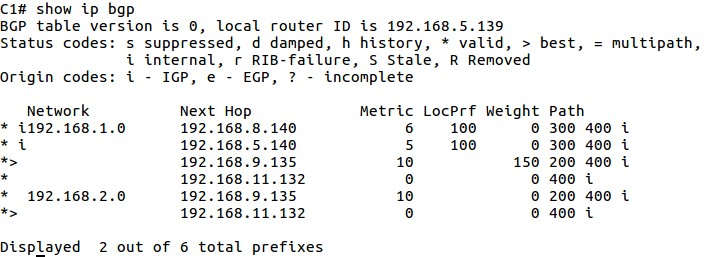
\includegraphics[width=0.8\textwidth]{c1-table}
  \caption{自治系统内全连接拓扑下C1的Loc-RIB表项}
  \label{fig:c1-table}
\end{figure}


\begin{figure}
  \centering
  % Requires \usepackage{graphicx}
  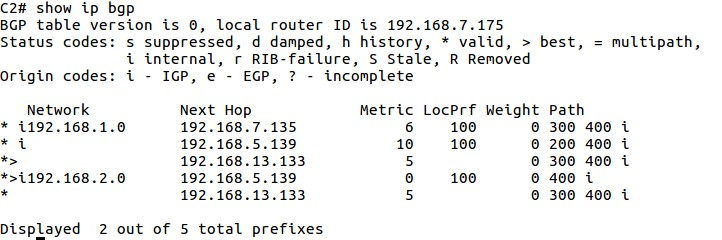
\includegraphics[width=0.8\textwidth]{c2-table}
  \caption{自治系统内全连接拓扑下C2的Loc-RIB表项}
  \label{fig:c2-table}
\end{figure}

\begin{figure}
  \centering
  % Requires \usepackage{graphicx}
  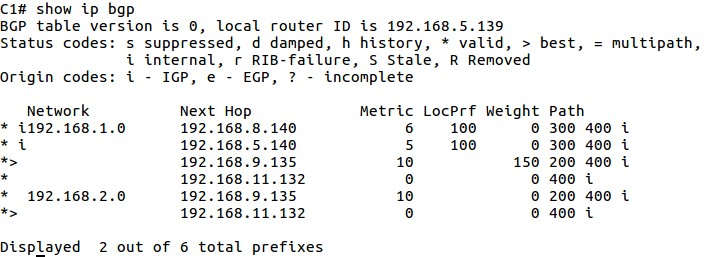
\includegraphics[width=0.8\textwidth]{c1-table}
  \caption{自治系统内全连接拓扑下C3的Loc-RIB表项}
  \label{fig:c3-table}
\end{figure}

%\begin{table}[]
%\centering
%\caption{自治系统内全连接拓扑下C2的Loc-RIB表项}
%\label{tab:c2-fm}
%\begin{tabular}{|c|c|c|c|c|c|c|}
%\hline
%Network     & \begin{tabular}[c]{@{}c@{}}Origin\\ code\end{tabular} & Next Hop          & Metirc & LocPrf & Weight & Aspaths   \\ \hline
%192.168.1.0 &                                                       & 192.168.13.133-R2  & 5      &        & 0      & 300 400 i \\ \hline
%            & i                                                     & 192.168.5.139-C1 & 10     & 100    & 0      & 200 400 i \\ \hline
%192.168.2.0 &                                                       & 192.168.13.133-R2 & 5      &        & 0      & 300 400 i \\ \hline
%            & i                                                     & 192.168.5.139-C1  & 0      & 100    & 0      & 400 i     \\ \hline
%\end{tabular}
%\end{table}


%\begin{table}[]
%\centering
%\caption{自治系统内全连接拓扑下C3的Loc-RIB表项}
%\label{tab:c3-fm}
%\begin{tabular}{|c|c|c|c|c|c|c|}
%\hline
%Network     & \begin{tabular}[c]{@{}c@{}}Origin\\ code\end{tabular} & Next Hop          & Metirc & LocPrf & Weight & Aspaths   \\ \hline
%192.168.1.0 & i                                                     & 192.168.7.175-C2  & 5      & 100    & 0      & 300 400 i \\ \hline
%            &                                                       & 192.168.14.131-R2 & 6      &        & 0      & 300 400 i \\ \hline
%            & i                                                     & 192.168.8.141-C1  & 10     & 100    & 0      & 200 400 i \\ \hline
%192.168.2.0 &                                                       & 192.168.14.131-R2 & 6      &        & 0      & 300 400 i \\ \hline
%            & i                                                     & 192.168.8.141-C1  & 0      & 100    & 0      & 400 i     \\ \hline
%\end{tabular}
%\end{table}


使用虚拟机搭建图\ref{fig:rscp-example1}的网络拓扑,自治系统号为100的自治系统外的边界路由器通过安装了Linux系统的虚拟机运行软件路由器Quagga来,自治系统号为100的自治系统内部部署RSCP-iBGP系统,自治系统号为100的自治系统内的边界路由器通过安装了Linux系统的虚拟机运行修改后的软件路由器Quagga-Route-Client来模拟,自治系统号为100的自治系统内的Route-Server路由器通过安装了Linux系统的虚拟机运行修改后的软件路由器Quagga-Route-Server来模拟。仍需要在R1、R2、C1上使用Route-map过滤更新策略,来配置BGP策略,使得从R1宣告给C1的路由MED值=10,从R2宣告给C2的路由MED=5,从R2宣告给C3的路由MED=6,从R1收到的Prefix192.168.1.0/24的路由信息经过C1的入站策略后该路由的Weight值改为150,通过iBGP协议传输的iBGP路由信息Local Preference默认为100。则当R3向外宣告192.168.1.0/24和192.168.2.0/24时,自治系统号为100的自治系统内Route-Server路由器上存储的Public-Loc-RIB见表\ref{tab:pub}。 因为192.168.1.0/24和192.168.2.0/24前缀的最优路由与Weight相关的仅有C1边界路由器,则Route-Server仅存储了针对C1的Private-Loc-RIB,见表\ref{tab:pri}。

\begin{table}[]
\centering
\caption{Route-Server路由器中的Public-Loc-RIB表项}
\label{tab:pub}
\begin{tabular}{|c|c|l|c|c|c|c|}
\hline
Network     & \begin{tabular}[c]{@{}c@{}}Received\\ iBGP-Peer\end{tabular} & Next Hop & Metric & LocPrf & Weight & Aspaths   \\ \hline
192.168.1.0 & C1                                                           & R3       & 0      & 100    &  /    & 400,i     \\ \hline
192.168.1.0 & C1                                                           & R1       & 10     & 100    & /    & 200,400,i \\ \hline
192.168.1.0 & C2                                                           & R2       & 5      & 100    &  /     & 300,400,i \\ \hline
192.168.1.0 & C3                                                           & R2       & 6      & 100    &   /     & 300,400,i \\ \hline
192.168.2.0 & C1                                                           & R3       & 0      & 100    &  /      & 400,i     \\ \hline
192.168.2.0 & C1                                                           & R1       & 10     & 100    &  /      & 200,400,i \\ \hline
192.168.2.0 & C2                                                           & R2       & 5      & 100    &  /      & 300,400,i \\ \hline
192.168.2.0 & C3                                                           & R2       & 6      & 100    &  /      & 300,400,i \\ \hline
\end{tabular}
\end{table}



\begin{table}[]
\centering
\caption{Route-Server路由器中的针对C1的Private-Loc-RIB表项}
\label{tab:pri}
\begin{tabular}{|c|c|l|c|c|c|c|}
\hline
Network     & \begin{tabular}[c]{@{}c@{}}Received\\ iBGP-Peer\end{tabular} & Next Hop & Metric & LocPrf & Weight & Aspaths   \\ \hline
192.168.1.0 & C1                                                           & R3       & 0      & 100    &      & 400,i     \\ \hline
192.168.1.0 & C1                                                           & R1       & 10     & 100    & 150    & 200,400,i \\ \hline
192.168.1.0 & C2                                                           & R2       & 5      & 100    &       & 300,400,i \\ \hline
192.168.1.0 & C3                                                           & R2       & 6      & 100    &        & 300,400,i \\ \hline
\end{tabular}
\end{table}


传统的Loc-RIB路由信息,存储于自治系统内部的边界路由器上。假设自治系统内有N台路由器,外部有M条路由传到该自治系统,则每台路由器存储约M条Loc-RIB路由表项,自治系统内总共存储约N*M条路由信息。在图\ref{fig:rscp-example-fm}的拓扑条件下,自治系统号为100的自治系统共存储了约N*M(N=3)条路由。而本文提出的RSCP-iBGP系统中只需存储一份M条表项的Public-Loc-RIB信息和若干份与Weight值相关的m条表项的前缀路由信息,则自治系统共存储M+m条路由信息,因为m远小于M,则自治系统共存储了约M条路由表项。在图\ref{fig:rscp-example1}的拓扑条件下,自治系统号为100的自治系统共存储了约M+m(m远小于M)条路由。相比于传统的分布式路由存储方式,本文提出的RSCP-iBGP系统中的增量路由存储将需要路由表项的总数下降了一个数量级,对路由存储进行了优化。


\subsection{路由计算集中优化}

在图\ref{fig:rscp-example-fm}的拓扑条件下,路由策略配置使得从R1宣告给C1的路由MED值=10,从R2宣告给C2的路由MED=5,从R2宣告给C3的路由MED=6,从R1收到的Prefix192.168.1.0/24的路由信息经过C1的入站策略后该路由的Weight值改为150,通过iBGP协议传输的iBGP路由信息Local Preference默认为100(路由比较过程中如果LocPrf值未设置,默认为100)。则当R3向外宣告192.168.1.0/24和192.168.2.0/24前缀时,C1、C2、C3分别根据自己收到的路由和路由策略,分别计算最优路由。最后,C1针对192.168.1.0/24前缀计算出的最优路由是C1-R1-R3, C1针对192.168.2.0/24前缀计算出的最优路由是C1-R3;C2针对192.168.1.0/24前缀计算出的最优路由是C2-R2-R3, C2针对192.168.2.0/24前缀计算出的最优路由是C2-C1-R3;C3针对192.168.1.0/24前缀计算出的最优路由是C3-R2-R3, C3针对192.168.2.0/24前缀计算出的最优路由是C3-C1-R3,总共计算了6次。若自治系统内有N台边界路由器,当一条更新路由传到自治系统时,每台边界路由器均需进行路由更新流程,如果最优路由发生变化则需要进行再次宣告,进入路由收敛过程,在这个过程中路由计算最少N次,最多N\verb+*+(N-1)/2次。


在图\ref{fig:rscp-example1}的拓扑条件下,路由策略配置使得从R1宣告给C1的路由MED值=10,从R2宣告给C2的路由MED=5,从R2宣告给C3的路由MED=6,从R1收到的Prefix192.168.1.0/24的路由信息经过C1的入站策略后该路由的Weight值改为150,通过iBGP协议传输的iBGP路由信息Local Preference默认为100(路由比较过程中如果LocPrf值未设置,默认为100)。则当R3向外宣告192.168.1.0/24和192.168.2.0/24前缀时,C1、C2、C3分别根据自己收到的路由传输到路由集中控制平台Route-Server路由器,Route-Server根据全部的路由信息为每一台边界路由器计算最优路由。针对192.168.1.0/24前缀,Route-Server通过Public-RIB-In计算一次得到C2和C3的最优出口,再通过针对C1的Private-RIB-In计算一次得到C1的最优出口。针对192.168.2.0/24前缀,Route-Server仅需计算一次即可得到C1、C2、C3的最优路由,因为192.168.2.0/24最优路由的决定性条件是Aspath长度,这属于所有边界路由器相同的可比路由属性。因为不存在路由收敛,所以当一条新路由传输到自治系统,RSCP-iBGP系统路由计算最少1次,最多N次。相比有路由收敛的传统分布式路由,本文提出的RSCP-iBGP将当新路由到达自治系统时,自治系统内的路由计算次数平均优化了一个数量级。

\subsection{基于全部路由且无MED值引起的路由震荡}


\begin{figure}
  \centering
  % Requires \usepackage{graphicx}
  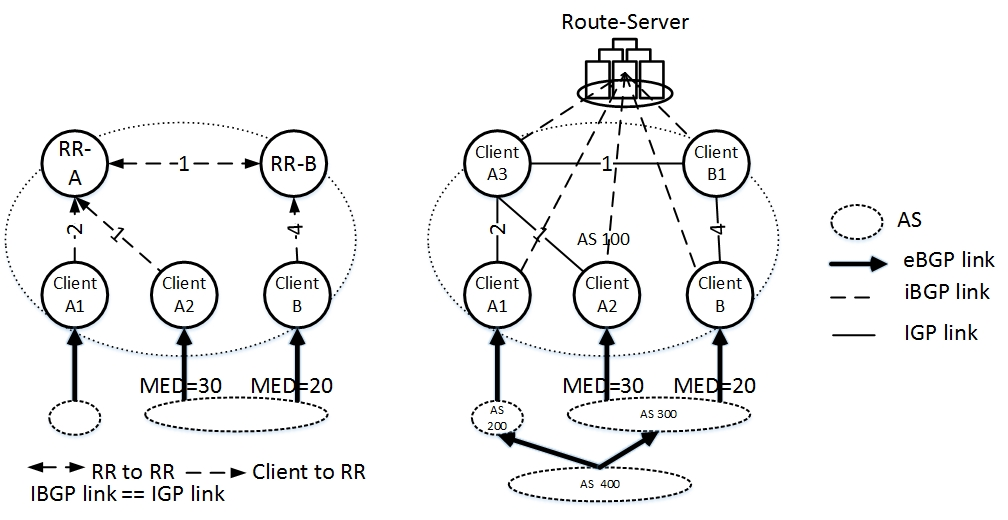
\includegraphics[width=0.75\textwidth]{rscp-fixmed}
  \caption{RSCP-iBGP系统下解决RR引起的MED路由震荡的实验拓扑}
  \label{fig:rscp-fixmed}
\end{figure}


本文提出的RSCP-iBGP系统中的复式路由计算,基于全部的路由进行计算。路由计算的过程采用集合排除法,当自治系统相同的时候,从Prefix的路由集合中删除MED值更大的路由,保证路由更新到达顺序不一致的情况下,最终当基于全部路由进行计算的时候,得到的最优路由是确定的。以RR路由反射引起的MED路由震荡为例,如图\ref{fig:rscp-fixmed}。

通过虚拟机搭建图\ref{fig:rscp-fixmed}中右侧拓扑的网络环境,AS400的边界路由器向外宣告192.168.1.0/24前缀。通过查看Route-Server路由存储情况,可以发现AS400向外宣告的192.168.1.0/24路由信息通过AS100的三个入口A1、A2、B传输到Route-Server,最后存储进入Route-Server放入Public-Loc-RIB表中。最终Route-Server通过复式路由计算算法,因为从A2、B口传输到集中平台的路由来源于AS300,则根据集合消除法的原则,消除A2进入的路由。最终A1、A2、B的针对192.168.1.0/24前缀的最优出口根据IGPcost选择。

该实验拓扑下,Route-Server上显示A1的针对192.168.1.0/24的最优出口为本身(AS200),A2的针对192.168.1.0/24的最优出口为A1,B的针对192.168.1.0/24的最优出口为本身(AS300)。实验结果证明,因为复式路由计算基于全部路由进行路由计算,且因为采取集合消除法非两两比较则不会发生MED路由震荡。



\section{协议的一致性测试}

\begin{figure}
  \centering
  % Requires \usepackage{graphicx}
  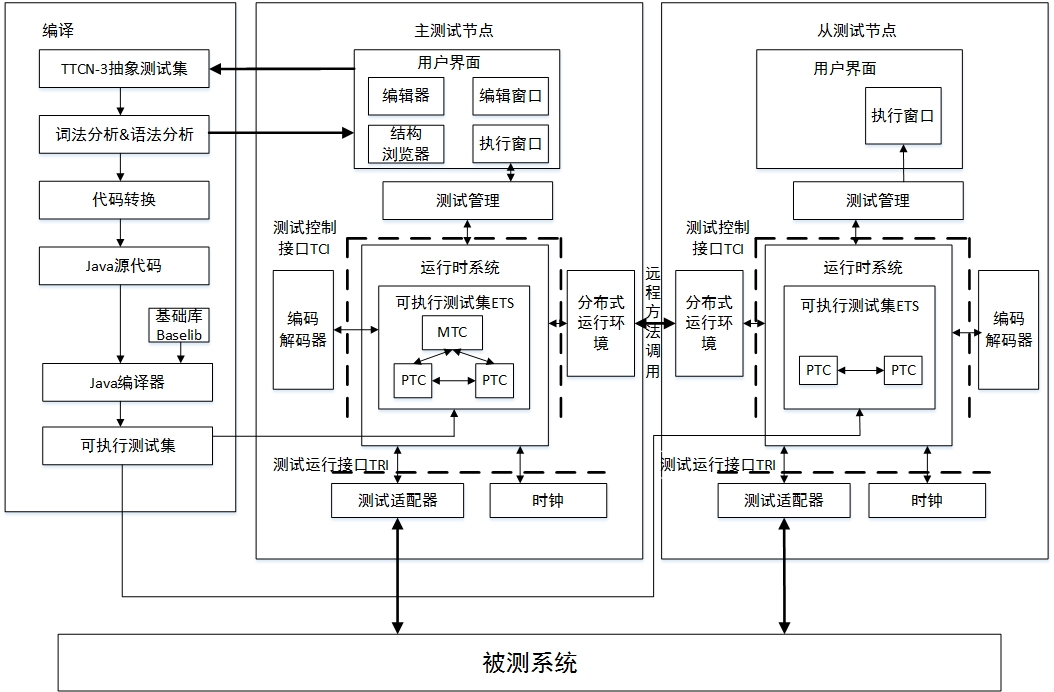
\includegraphics[width=0.75\textwidth]{pitsv3}
  \caption{PitSv3系统的体系结构\cite{journals_chinaf_YinWJS08}}
  \label{fig:pitsv3}
\end{figure}

\subsection{测试平台介绍}
测试平台使用协议测试系统工具PITSv3\cite{journals_chinaf_YinWJS08}(Protocol Integrated Test System Version 3),PITSv3内通过主测试部件和多个从测试部件,来模拟测试系统多网口的情况,每个测试部件可以连接一个真实的虚拟路由器,以此来构建测试系统连接的网络拓扑,从而实现对协议的一致性测试。PITSv3系统的体系结构见图\ref{fig:pitsv3}。

本文中针对RSCP-iBGP系统的功能测试,依托安装在物理机器上的VMware Workstation Pro虚拟机管理软件,在VMware虚拟机管理软件中运行多台虚拟机,分别作为(安装PITSv3的Windows系统)测试系统和(运行RSCP-iBGP系统中的Route-Client软件路由器或者Route-Server软件路由器的Linux系统)被测系统\cite{pitsv3}。

\subsection{一致性测试需求}

对RSCP-iBGP系统的测试主要分两个测试部分:对自治系统内的边界路由器Route-Client进行测试,对自治系统内的Route-Server进行测试,具体的测试需求如下。

% Please add the following required packages to your document preamble:
% \usepackage{multirow}
\begin{table}[]
\centering
\caption{RSCP-iBGP系统中Route-Client与eBGP邻居的一致性测试集}
\label{tab:test1}
\begin{tabular}{|c|c|l|}
\hline
测试组                                  & 测试用例     & 测试目的                                                                         \\ \hline
\multirow{4}{*}{Route-Client与eBGP邻居} & 邻居建连测试   & \begin{tabular}[c]{@{}l@{}}Route-Client可以接收\\ eBGP邻居的主动连接\end{tabular}       \\ \cline{2-3}
                                     & 对等体断连测试  & \begin{tabular}[c]{@{}l@{}}Route-Client可以处理\\ eBGP邻居的主动断连\end{tabular}       \\ \cline{2-3}
                                     & 前缀报文接收测试 & \begin{tabular}[c]{@{}l@{}}Route-Client可以收到\\ eBGP邻居的UPDATE报文\end{tabular}   \\ \cline{2-3}
                                     & 前缀报文处理测试 & \begin{tabular}[c]{@{}l@{}}Route-Client将eBGP邻居的路由更新\\ 附加Weight属性发给iBGP邻居\end{tabular} \\ \hline
\end{tabular}
\end{table}


\subsubsection{被测系统Route-Client与eBGP邻居之间的测试}

被测系统Route-Client与eBGP邻居,进行eBGP邻居建连测试、eBGP对等体断连测试、eBGP对等体前缀报文接收测试、eBGP对等体前缀报文处理测试:
\begin{itemize}
  \item 被测系统Route-Client与eBGP邻居,进行eBGP邻居建连测试:测试系统软件向Route-Client被测系统发送OPEN报文,请求与Route-Client建立eBGP连接,当测试系统软件收到被测系统Route-Client回复过来的OPEN报文和KEEPALIVE报文,表明eBGP邻居建连成功;
  \item 被测系统Route-Client与eBGP邻居,进行eBGP对等体断连测试:测试系统软件向Route-Client被测系统发送OPEN报文,请求与Route-Client建立eBGP连接,当测试系统软件收到被测系统Route-Client回复过来的OPEN报文和KEEPALIVE报文,则邻居建连成功,测试系统回复KEEPALIVE报文维持连接,之后测试系统主动断开BGP连接,即连续三次收到Route-Client被测系统发来的KEEPALIVE不回复,最后测试系统收到了Route-Client被测系统通知断连的NOTIFICATION报文,表明eBGP对等体断连成功;
  \item 被测系统Route-Client与eBGP邻居,进行eBGP对等体前缀报文接收测试:测试系统软件和Route-Client被测系统建立eBGP连接,测试系统软件通过向Route-Client被测系统发送UPDATE报文信息,如果Route-Client被测系统正确接收到eBGP报文,Route-Client开启该eBGP对等体的Adj-RIB-In存储的情况下,能够查到收到的UPDATE报文信息,表明eBGP对等体前缀报文接收成功;
  \item 被测系统Route-Client与eBGP邻居,进行eBGP对等体前缀报文处理测试:测试系统软件端口A和Route-Client被测系统建立eBGP连接,测试系统软件端口B和Route-Client被测系统建立iBGP连接。测试系统软件端口A通过向Route-Client被测系统发送UPDATE报文信息,如果Route-Client被测系统正确接收到eBGP报文,Route-Client开启该eBGP对等体的Adj-RIB-In存储的情况下,能够查到收到的UPDATE报文信息,表明eBGP对等体前缀报文接收成功;此时测试系统端口B收到了Route-Client发过来的携带Weight属性信息的UPDATE报文(配置Route-Client被测系统从某eBGP对等体收到路由的Weight值),表明eBGP对等体前缀报文处理正确。
\end{itemize}


\begin{table}[]
\centering
\caption{RSCP-iBGP系统中Route-Client与iBGP邻居的一致性测试集}
\label{tab:test2}
\begin{tabular}{|c|c|l|}
\hline
测试组                                  & 测试用例     & 测试目的                                                                         \\ \hline
\multirow{4}{*}{Route-Client与iBGP邻居} & 邻居建连测试   & \begin{tabular}[c]{@{}l@{}}Route-Client可以接收\\ iBGP邻居的主动连接\end{tabular}       \\ \cline{2-3}
                                     & 对等体断连测试  & \begin{tabular}[c]{@{}l@{}}Route-Client可以处理\\ iBGP邻居的主动断连\end{tabular}       \\ \cline{2-3}
                                     & 前缀报文接收测试 & \begin{tabular}[c]{@{}l@{}}Route-Client可以收到\\ iBGP邻居的UPDATE报文\end{tabular}   \\ \cline{2-3}
                                     & 前缀报文处理测试 & \begin{tabular}[c]{@{}l@{}}Route-Client可将iBGP邻居\\ 的路由更新宣告给所有eBGP邻居\end{tabular} \\ \hline
\end{tabular}
\end{table}

\subsubsection{被测系统Route-Client与iBGP邻居之间的测试}

被测系统Route-Client与iBGP邻居,进行iBGP邻居建连测试、iBGP对等体断连测试、iBGP对等体前缀报文接收测试、iBGP对等体前缀报文处理测试:
\begin{itemize}
  \item 被测系统Route-Client与iBGP邻居,进行iBGP邻居建连测试:测试系统软件向Route-Client被测系统发送OPEN报文,请求与Route-Client建立iBGP连接,当测试系统软件收到被测系统Route-Client回复过来的OPEN报文和KEEPALIVE报文,表明iBGP邻居建连成功;
  \item 被测系统Route-Client与iBGP邻居,进行iBGP对等体断连测试:测试系统软件向Route-Client被测系统发送OPEN报文,请求与Route-Client建立iBGP连接,当测试系统软件收到被测系统Route-Client回复过来的OPEN报文和KEEPALIVE报文,则邻居建连成功,测试系统回复KEEPALIVE报文维持连接,之后测试系统主动断开BGP连接,即连续三次收到Route-Client被测系统发来的KEEPALIVE不回复,最后测试系统收到了Route-Client被测系统通知断连的NOTIFICATION报文,表明iBGP对等体断连成功;
  \item 被测系统Route-Client与iBGP邻居,进行iBGP对等体前缀报文接收测试:测试系统软件和Route-Client被测系统建立iBGP连接,测试系统软件通过向Route-Client被测系统发送UPDATE报文信息,如果Route-Client被测系统正确接收到iBGP报文,Route-Client开启该iBGP对等体的Adj-RIB-In存储的情况下,能够查到收到的UPDATE报文信息,表明iBGP对等体前缀报文接收成功;
  \item 被测系统Route-Client与iBGP邻居,进行iBGP对等体前缀报文处理测试:测试系统软件端口A和Route-Client被测系统建立eBGP连接,测试系统软件端口B和Route-Client被测系统建立eBGP连接,测试系统软件端口C和Route-Client被测系统建立iBGP连接。测试系统软件端口C通过向Route-Client被测系统发送UPDATE报文信息,如果Route-Client被测系统正确接收到iBGP报文,Route-Client开启该iBGP对等体的Adj-RIB-In存储的情况下,能够查到收到的UPDATE报文信息,表明iBGP对等体前缀报文接收成功;此时测试系统端口A和B收到了Route-Client转发过来的从iBGP收到的前缀的最优路由的UPDATE报文,表明iBGP对等体前缀报文,表明iBGP对等体前缀报文处理正确。
\end{itemize}





\begin{table}[]
\centering
\caption{RSCP-iBGP系统中Route-Server与iBGP邻居的一致性测试集}
\label{tab:test3}
\begin{tabular}{|c|c|l|}
\hline
测试组                                  & 测试用例     & 测试目的                                                                         \\ \hline
\multirow{4}{*}{\begin{tabular}[c]{@{}c@{}}Route-Server与\\ iBGP邻居\end{tabular}} & 邻居建连测试   & \begin{tabular}[c]{@{}l@{}}Route-Server可以接收\\ iBGP邻居的主动连接\end{tabular}       \\ \cline{2-3}
                                     & 对等体断连测试  & \begin{tabular}[c]{@{}l@{}}Route-Server可以处理\\ iBGP邻居的主动断连\end{tabular}       \\ \cline{2-3}
                                     & 前缀报文接收测试 & \begin{tabular}[c]{@{}l@{}}Route-Server可以收到iBGP邻居\\ 的带Weight属性值的UPDATE报文\end{tabular}   \\ \cline{2-3}
                                     & 前缀报文处理测试 & \begin{tabular}[c]{@{}l@{}}Route-Server收到iBGP邻居的路由更新,计算\\ iBGP邻居对应最优路由并宣告给每个iBGP邻居\end{tabular} \\ \hline
\end{tabular}
\end{table}

\subsubsection{被测系统Route-Server与iBGP邻居之间的测试}

被测系统Route-Server与iBGP邻居,进行iBGP邻居建连测试、iBGP对等体断连测试、iBGP对等体前缀报文接收测试、iBGP对等体前缀报文处理测试:
\begin{itemize}
  \item 被测系统Route-Server与iBGP邻居,进行iBGP邻居建连测试:测试系统软件向Route-Server被测系统发送OPEN报文,请求与Route-Server建立iBGP连接,当测试系统软件收到被测系统Route-Server回复过来的OPEN报文和KEEPALIVE报文,表明iBGP邻居建连成功;
  \item 被测系统Route-Server与iBGP邻居,进行iBGP对等体断连测试:测试系统软件向Route-Server被测系统发送OPEN报文,请求与Route-Server建立iBGP连接,当测试系统软件收到被测系统Route-Server回复过来的OPEN报文和KEEPALIVE报文,则邻居建连成功,测试系统回复KEEPALIVE报文维持连接,之后测试系统主动断开BGP连接,即连续三次收到Route-Server被测系统发来的KEEPALIVE不回复,最后测试系统收到了Route-Server被测系统通知断连的NOTIFICATION报文,表明iBGP对等体断连成功;
  \item 被测系统Route-Server与iBGP邻居,进行iBGP对等体前缀报文接收测试:测试系统软件和Route-Server被测系统建立iBGP连接,测试系统软件通过向Route-Server被测系统发送UPDATE报文信息,如果Route-Server被测系统正确接收到携带Weight属性信息的UPDATE报文,表明iBGP对等体前缀报文接收成功;
  \item 被测系统Route-Server与iBGP邻居,进行iBGP对等体前缀报文处理测试:测试系统软件端口A和Route-Server被测系统建立iBGP连接,测试系统软件端口B和Route-Server被测系统建立iBGP连接,测试系统软件端口C和Route-Server被测系统建立iBGP连接。测试系统软件端口A通过向Route-Server被测系统发送2条相同前缀不同路由的UPDATE报文信息,如果Route-Server被测系统正确接收到该2条路由信息,表明iBGP对等体前缀报文接收成功;此时测试系统端口A、B和C收到了Route-Server被测系统发来的该前缀的最优路由的UPDATE报文,表明被测系统Route-Server与iBGP对等体之间的前缀报文处理正确。
\end{itemize}



\subsection{测试集设计}

本文提出的RSCP-iBGP系统在自治系统内部有两种类型的路由器Route-Client边界路由器和Route-Server路由集中控制平台上的,Route-Client路由器有eBGP对等体和iBGP对等体,而Route-Server路由器仅有iBGP对等体。根据测试需求设计三组测试集共3组:Route-Client与eBGP邻居之间的一致性测试集如表\ref{tab:test1}、Route-Client与iBGP邻居之间的一致性测试集如表\ref{tab:test2}、Route-Server与iBGP邻居之间的一致性测试集如表\ref{tab:test3}。



\subsection{测试结果及分析}


\begin{figure}
  \centering
  % Requires \usepackage{graphicx}
  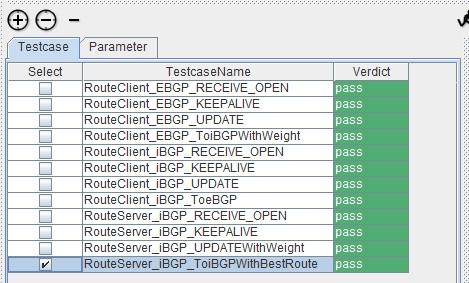
\includegraphics[width=0.8\textwidth]{test}
  \caption{被测系统Route-Client与eBGP邻居之间测试集的测试结果图}
  \label{fig:test}
\end{figure}


针对以上的测试需求和测试方案,本文对3组测试集进行了测试,被测系统Route-Client与eBGP邻居之间的测试软件中的结果如图\ref{fig:test}。3组测试集的测试例共12个进行测试,测试结果如表\ref{tab:res},从表中我们可以看出测试例全部通过。RSCP-iBGP系统中的Route-Client路由器和Route-Server可以进行正常的BGP协议下的报文交互,Route-Client路由器收到eBGP路由,会将其经过入站策略且携带Weight属性的路由信息传输到路由集中平台上的Route-Server路由器,Route-Server会计算出每台边界路由器针对该Prefix的最优路由,并将其传输给域内的每一台边界路由器Route-Client,之后Route-Client将收到的iBGP路由宣告给所有的eBGP邻居,整个路由处理的流程在RSCP-iBGP系统中均正确无误,证明RSCP-iBGP系统实现与设计规范的一致性。


% Please add the following required packages to your document preamble:
% \usepackage{booktabs}
\begin{table}[]
\centering
\caption{RSCP-iBGP系统一致性测试集的测试结果}
\label{tab:res}
\begin{tabular}{@{}ccc@{}}
\toprule
测试集名称               & 通过用例数 & 失败用例数 \\ \midrule
Route-Client与eBGP邻居 & 4     & 0     \\
Route-Client与iBGP邻居 & 4     & 0     \\
Route-Server与iBGP邻居 & 4     & 0     \\
总计                  & 12    & 0     \\ \bottomrule
\end{tabular}
\end{table}


\section{本章小结}

本章主要对RSCP-iBGP系统的进行了功能验证、BGP扩展协议一致性测试。通过本章的仿真实验和协议测试,本文实现的RSCP-iBGP系统在功能实现上达到了最初的设计目标:基于全部路由进行路由计算,集合缩小式的新型路由算法也能避免MED不可比引起的路由震荡,路由表在集中平台上存储优化。在本文提出的RSCP-iBGP系统中,自治系统内部的路由计算次数和路由存储大小均优化了一个数量级,且不存在路由震荡和路由收敛等情况。
